
\chapter{Related Works}
This work builds ontop of the 3D-Gaussian Splatting for Radiance Field Rendering Paper \cite{kerbl3Dgaussians}. Following existing point cloud transformers \cite{yu2021pointbert, \cite{yu2021pointr}} it uses a 


I will also mention the similarity to vision transformers such as:
\cite{devlin2019bert}
\cite{yu2021diverse}
\cite{Miao2024}

\chapter{Introduction}
While there are existing techniques for completing and reconstructing incomplete 3D point clouds, these only focus on the underlying geometry \cite{dai2020sgnn, song2016ssc, roldao20213d, yu2021pointr, yu2021pointbert}. Meanwhile vision transformers have shown great results in 2D image inpainting tasks \cite{Miao2024, yu2021diverse}. This thesis bridges the gap between these two fields by proposing a network that completes an incomplete point cloud geometry while filling in the missing visual information at the same time. This is done by directly predicting 3D-Gaussians. 3D-Gaussians are a sparse volumetric rendering method, by sampling points along rays a pixel value is calculated by using the properties of the Gaussians along the ray.\cite{article, kerbl3Dgaussians} So by predicting a Gaussians as whole it becomes possible to simultaneously complete the missing geometries and visuals for a scene.
\begin{figure}[h]
\centering % zentriert alles in der Figure
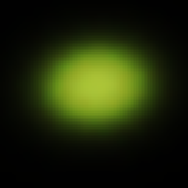
\includegraphics[width=0.262\linewidth]{Images/Chapter/A Gaussian.pdf} % externe Grafik laden
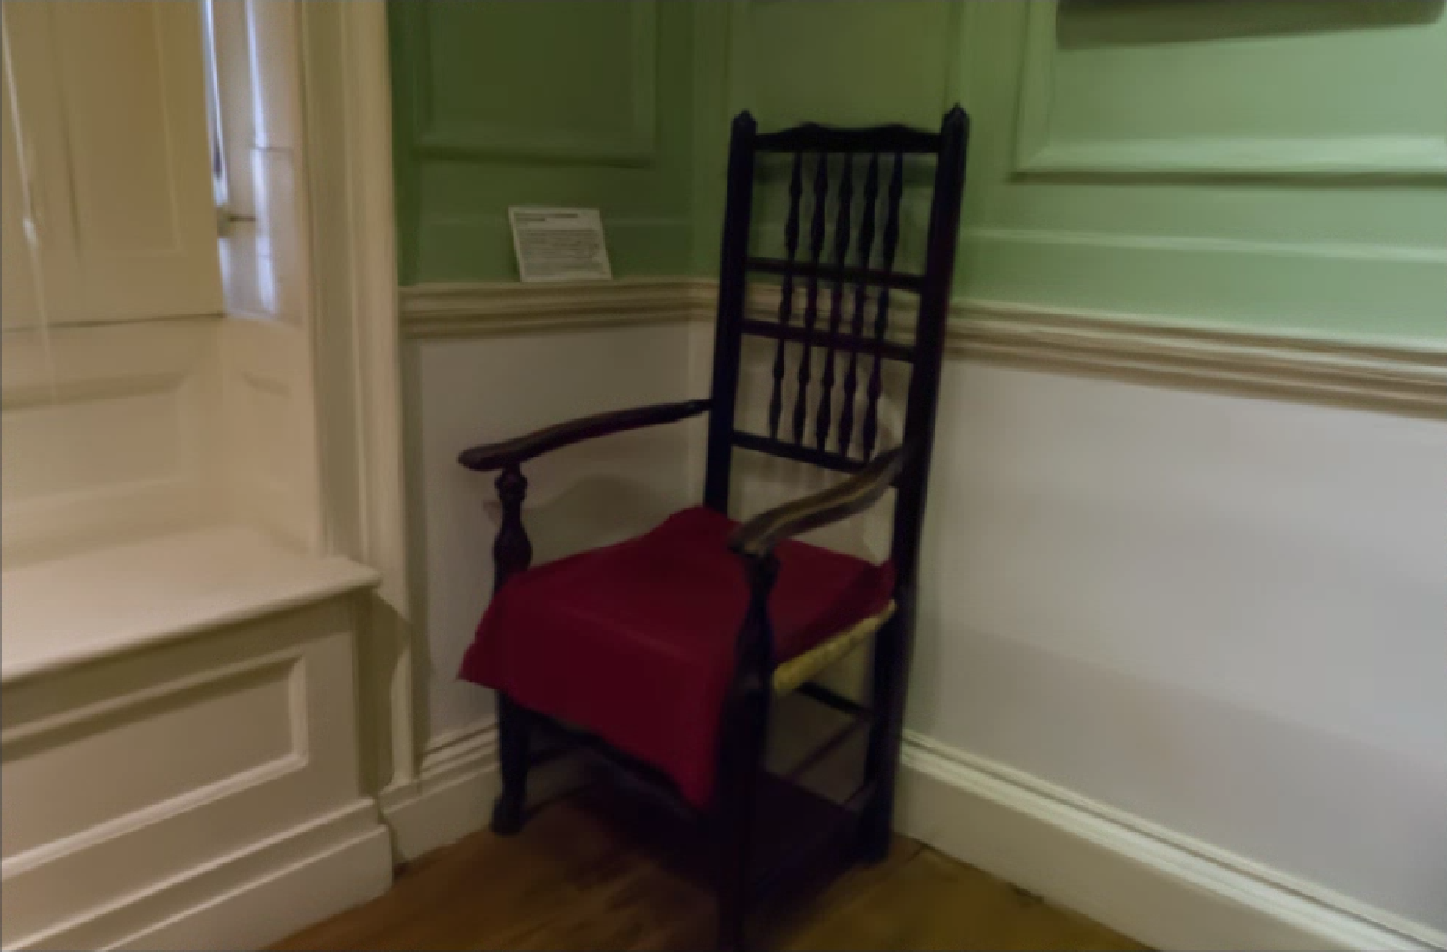
\includegraphics[width=0.4\linewidth]{Images/Chapter/chair.pdf}
\caption{A single Gaussian (left). Multiple Gaussians creating the image of a chair (right)}\label{fig:gaussians}
\end{figure}\\
\section{Motivation}
Optimizing a 3D-Gaussian Model begins by taking pictures from different positions with different camera angles. A structure from motion (SfM) program, such as Colmap \cite{schoenberger2016mvs, schoenberger2016sfm}, is then used to extract image features and place these features in a 3D space by matching the same features visible in different images. During this process the original camera positions and angles are recovered aswell \ref{fig:colmap}.\\
\begin{figure}[h]
\centering % zentriert alles in der Figure
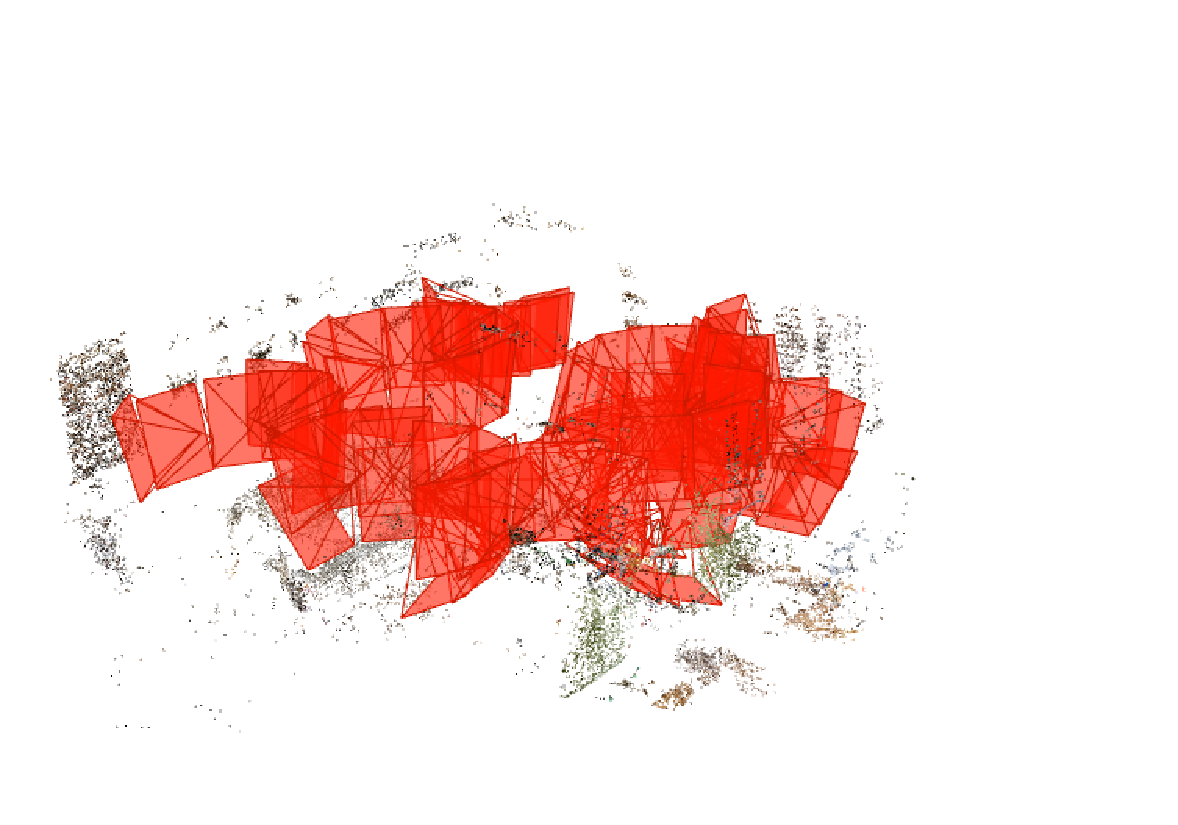
\includegraphics[width=0.6\linewidth]{Images/Chapter/colmap.pdf} % externe Grafik laden
\caption{A scene reconstruction in Colmap}\label{fig:colmap}
Cameras shown in red, features places in space.
\end{figure}
A sparse 3D-Gaussian Model is initialized using the extracted features and is then optimized using the original images as targets.
When viewing the resulting the resulting Model from novel viewpoints the quality of the rendered image depends strongly on how close the nearest training camera angles are. This makes the novel view synthesis is comparable to a 3D interpolation.\cite{kerbl3Dgaussians}\\
Subsequently if a part of the scene is not sufficiently covered in the original images holes or artifacts may appear in the scene for which no novel views can be synthesized due to lack of gaussians in the area (\ref{fig:hole}.\\
\begin{figure}[b]
\centering % zentriert alles in der Figure
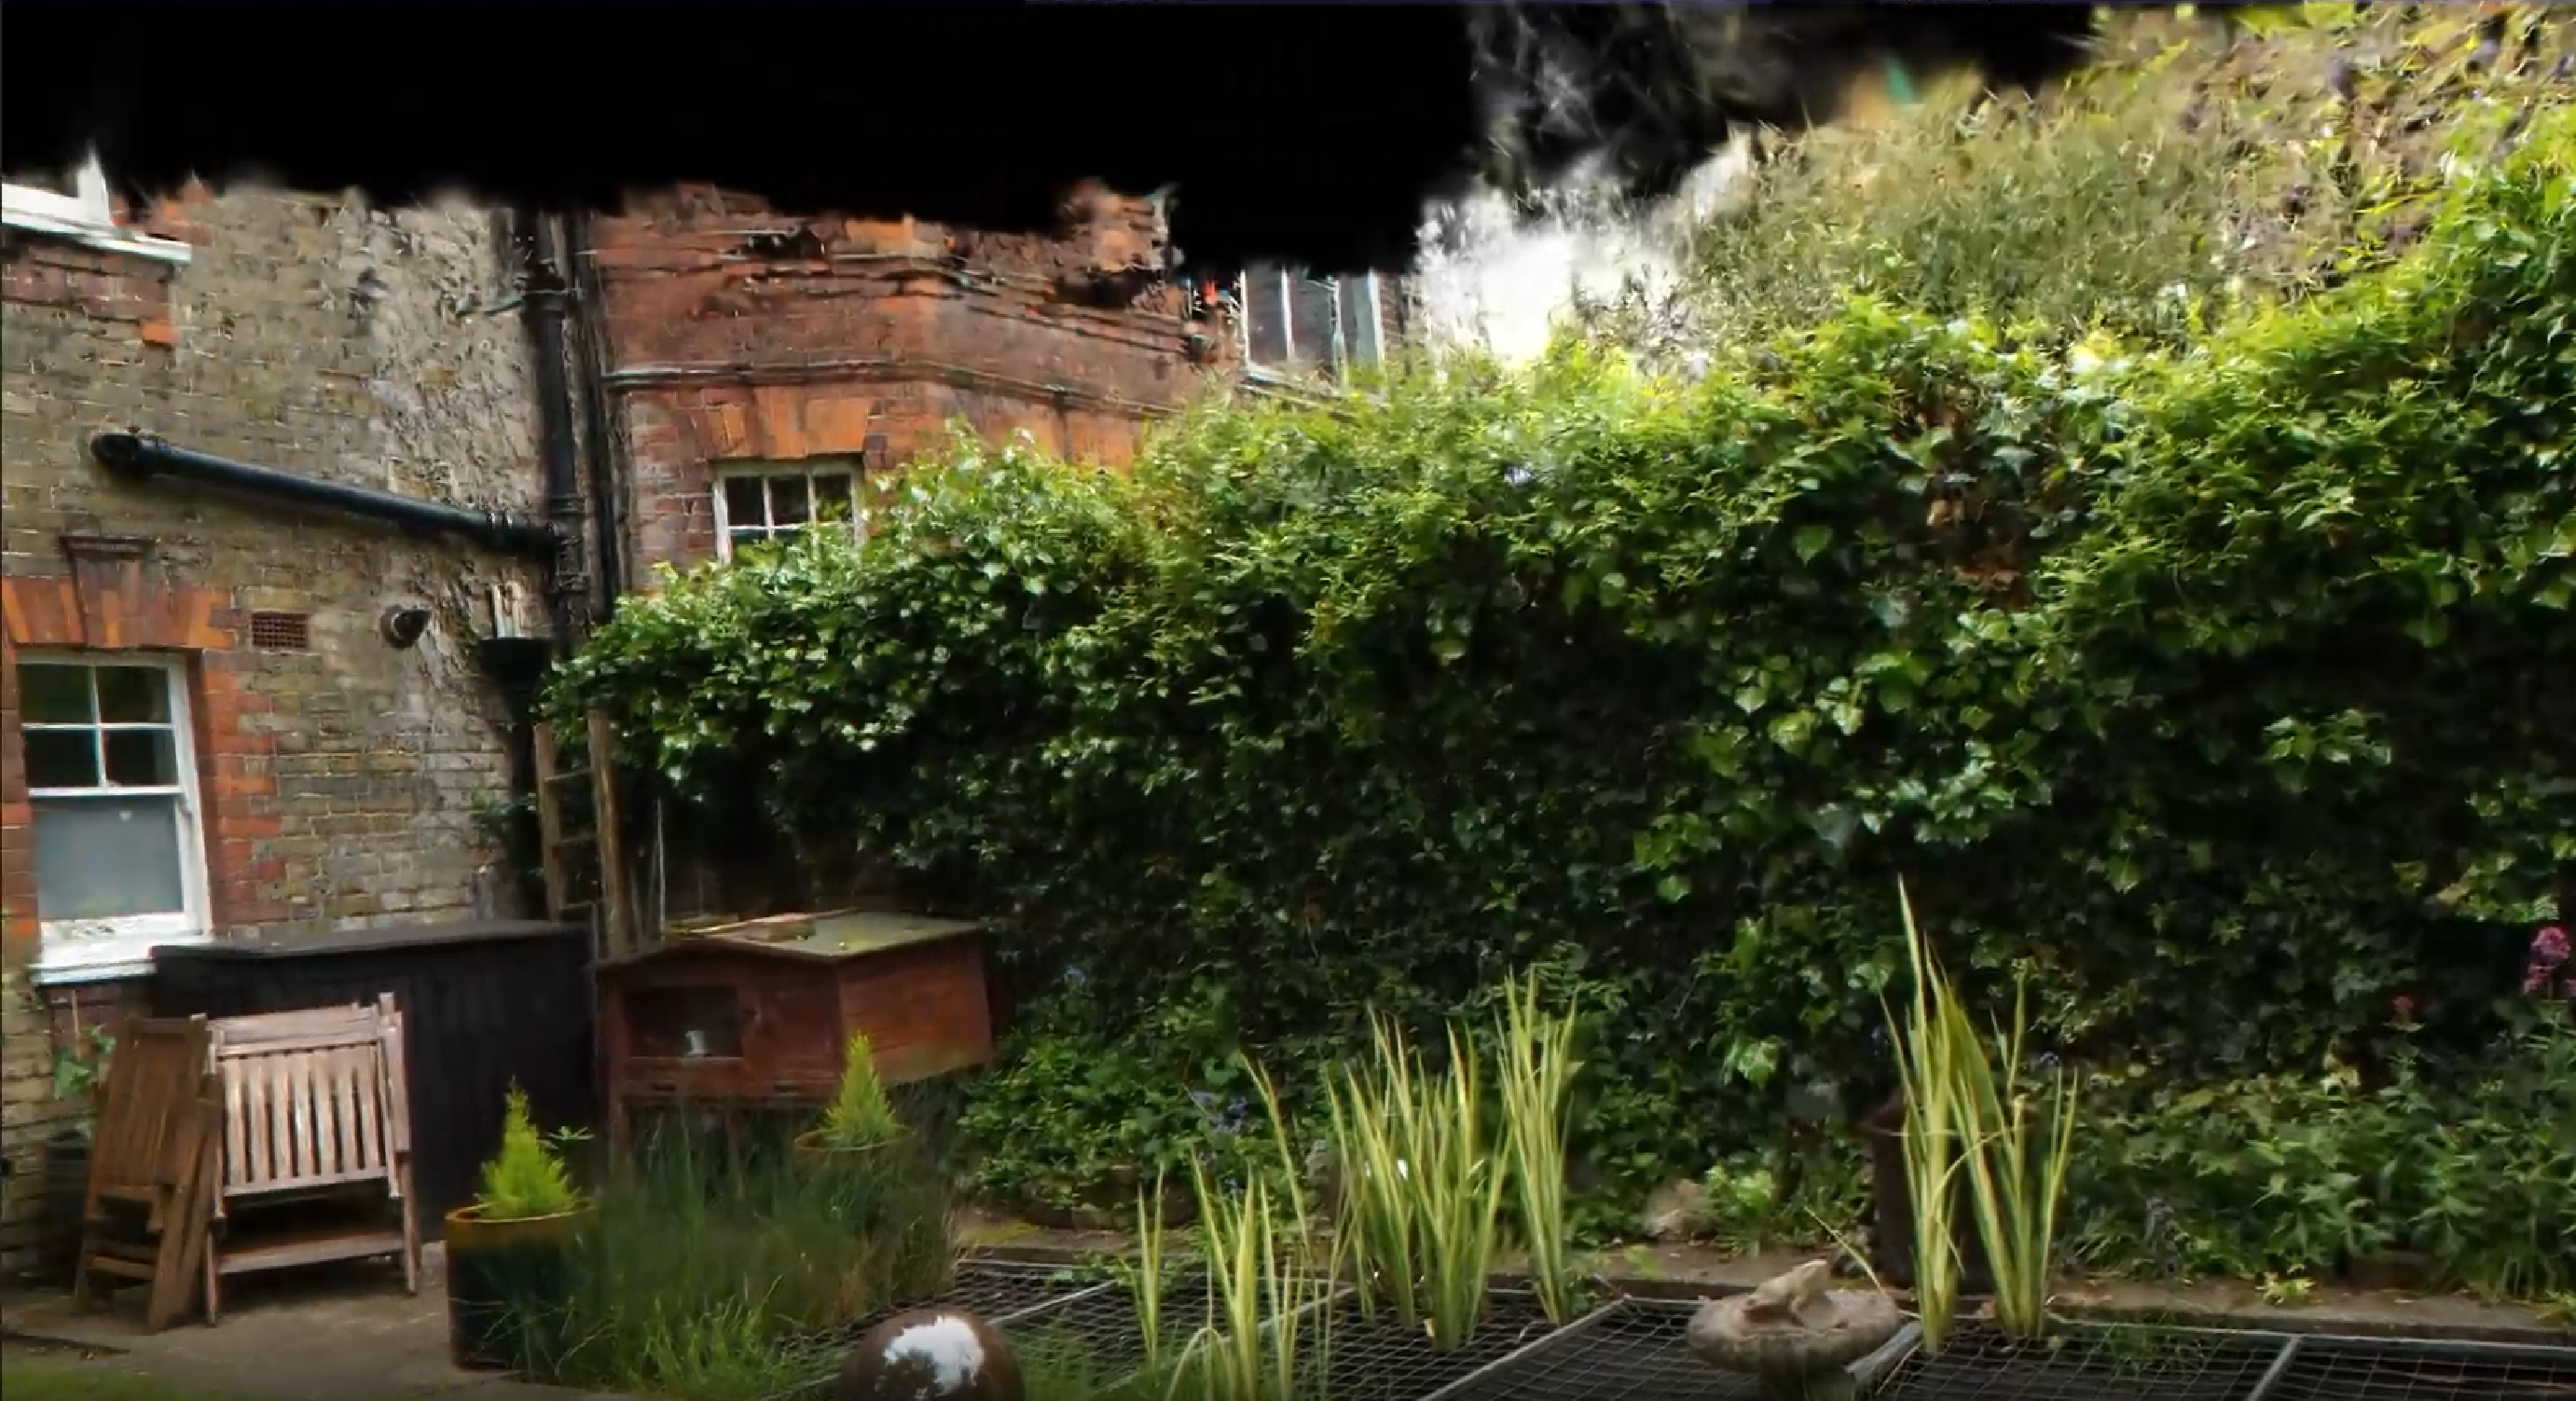
\includegraphics[width=0.6\linewidth]{Images/Chapter/hole.pdf} % externe Grafik laden
\caption{A Gaussian Model with missing parts at the top}\label{fig:hole}
\end{figure}
Currently there is no method to improve an already optimized 3D-Gaussian Model beyond adding more cameras and resuming training.\\
With the growing interest in using Gaussians as a 3D-Representation \cite{chen2024survey} it will become increasingly important to be able to work on Gaussians directly without referring back to the original images.\\
A semantic understanding of Gaussians would enable tasks such as compositing different Gaussian Models (e.g. placing a smaller object in a larger scene), segmenting a larger scene into smaller individual Models and completing or repairing an incomplete or faulty scene.
\section{Goals}
The goals of this work are as follows:\\
\begin{itemize}
    \item Encode an optimized but incomplete Gaussian Model with a transformer.
    \item Train the transformer to infer where the scene is missing Gaussians.
    \item Predict the missing geometries and visual data based on the rest of the scene.
    \item Decode the predicted geometries and visual data back into Gaussians
\end{itemize}

\section{Challenges}
Both encoding and decoding a Gaussian model are non-trivial tasks. For one the discrete, non-structural, and high-dimensional nature of 3D Gaussians make it difficult to predict their attributes directly \cite{zou2023triplane}.\\
Additionally a Gaussian Model very quickly is comprised of hundreds of thousands of Gaussians. This makes it computationally unfeasible to directly input every Gaussian into a transformer architecture, due to the quadratic memory demands of the Attention Layers used within. \cite{beltagy2020longformer}\\
Lastly the varying size of Gaussians leads to a non-homogeneous point cloud which makes it harder to sample from and understand the resulting geometries.\ref{fig:chairshrunk}
\begin{figure}
\centering % zentriert alles in der Figure
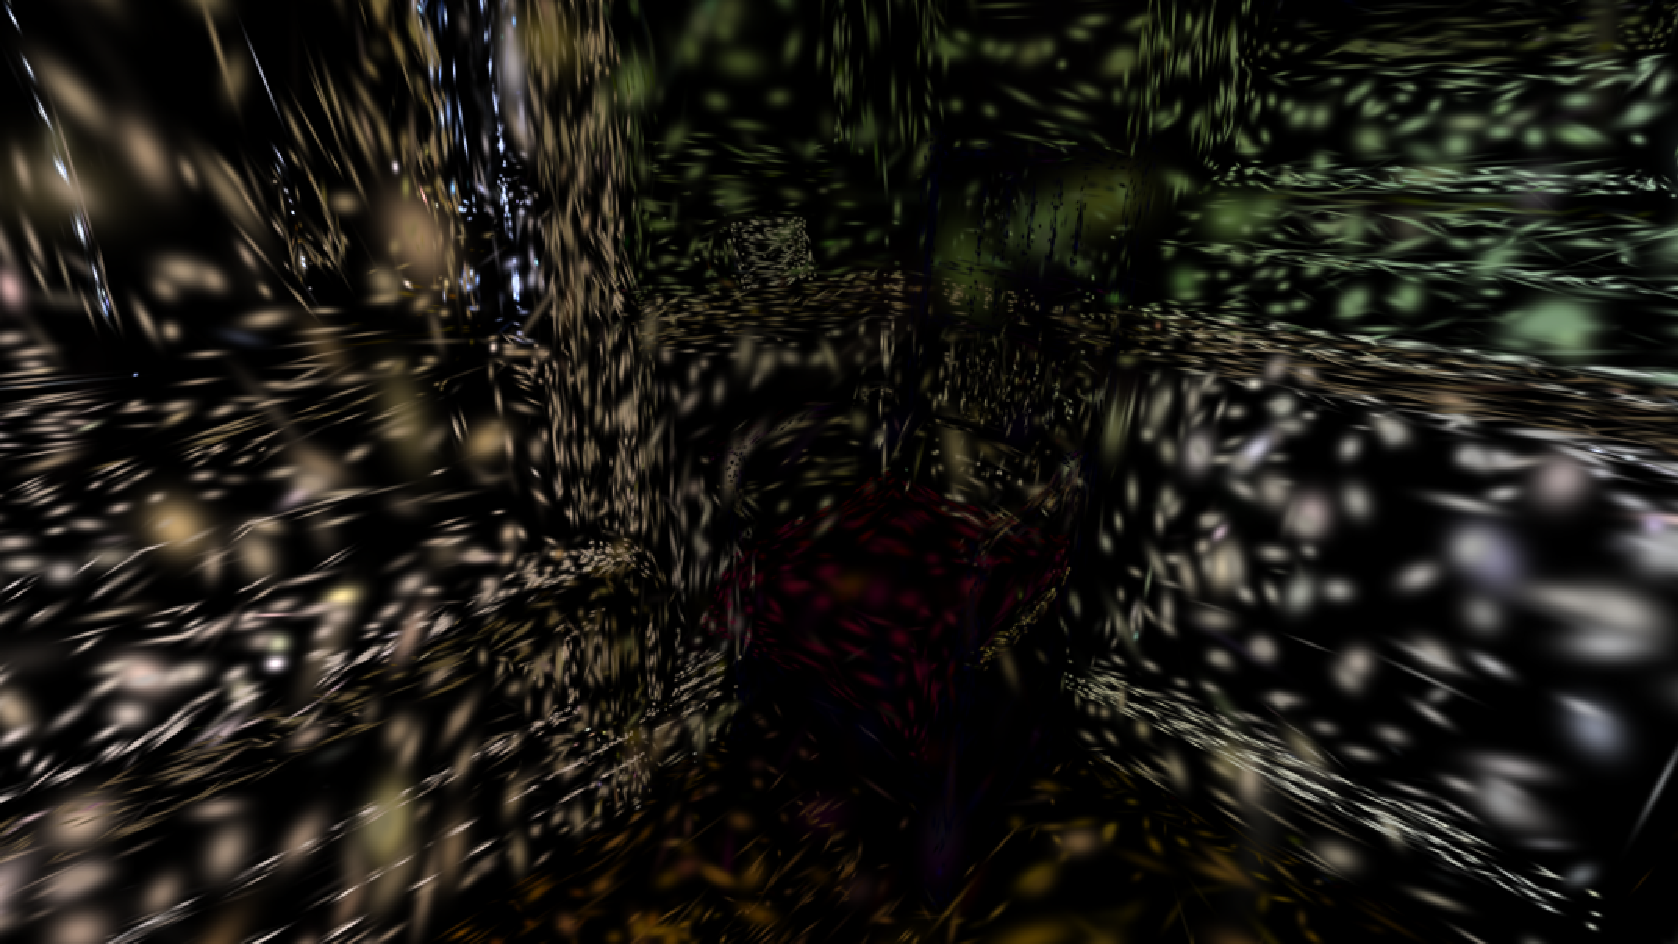
\includegraphics[width=0.6\linewidth]{Images/Chapter/chairshrunk.pdf} % externe Grafik laden
\caption{The chair from \ref{fig:gaussians} with scaled down Gaussians}\label{fig:chairshrunk}
After scaling down the Gaussian the different sizes and subsequently densities of throughout the scene become more apparent.
\end{figure}

\chapter{Network Architecture}
This chapter will start of with a diagram and description of the rough structure of the entire network.

\section{Visual Embedding}
This section will describe the Visual Embedding Net with a more closed up diagram. Both the novel encoder and the decoder (same as used in \cite{zou2023triplane}) will be elaborated on.
There will also be some pictures showing the capabilities of the Visual to encode and decode gaussians while retaining good image quality.

\section{DVAE}
This chapter will introduce the DVAE \cite{rolfe2017discrete} as a way comprehend a local pointcloud and convert it to a token and vice-versa.
\subsection{Sampling/Grouping}
This section will elaborate on the underwhelming performance of the commonly used Furthest-Point + KNN Sampling and will compare and contrast it with Random-Point + KNN Sampling.
\subsection{DGCNN}
This section will explain the DGCNN \cite{wang2019dynamic} and how it enables the DVAE to understand local geometries
\subsection{Discretization}
This section will introduce the vocabulary/codebook and how Gumbel-Softmax \cite{jang2017categorical} is used to discretize the resulting logits before sampling from the vocabulary.
\section{Transformer}
This section will talk about the transformer as a whole.
\subsection{Encoder}
This subsection will describe the self-attention mechanism and the positional encoding used in the encoder-blocks of the transformer.
\subsection{Query Generator}
This subsection will describe the Query generator as a way to turn the memory tokens generated by the encoder into positional information of where the missing content is located.
\subsection{Decoder}
This subsection will describe the cross-attention mechanism used to combine the memory and missing content tokens into useful output tokens.
\chapter{Training}
This chapter will explain the training regime used for the transformer. Describing both methods: 1. Training everything together vs 2. Training every component seperately 
\chapter{Results}
This chapter will look at some results, evaluating them both qualitatively and quantitavely. 
\section{Overall Evaluation}
This subsection will focus on the final results obtained.
\section{Vocabulary Analysis}
This subsection will analyze the different tokens learned by the DVAE.

\chapter{Limitations}
This chapter will highlight the limitations currently present in both the architecture and also results obtained

\chapter{Further Work}
\section{Improvements}
This chapter will somewhat speculate on ways that the architecture could be improved and goals i have in mind for future work on this particular problem
\section{Prospects}
This chapter will talk about the things that would become possible if I can achieve a good latent space representation of Gaussian Scenes (such as style-transfer, etc). 






% \subsubsection{Vierte Gliederungsebene}

% Drei Gliederungsebenen sollten für kleine Artikel und Ausarbeitungen genügen. 
% Anderenfalls sollte die Strukturierung nocheinmal überdacht werden.

% \paragraph{Paragraph ist die unterste Ebene} \blindtext

% \section{Tabellen einbinden}

% \begin{table}
% \centering
% \begin{tabular}{|c||lr|}\hline
% 1.1 & 1.2 & 1.3 \\ \hline
% 2.1 & 2.2 & 2.3 \\ \hline \hline
% 3.1 & 3.2 & 3.3 \\ \hline
% \end{tabular}
% \caption{Eine simple Tabelle}\label{tab:simple}
% \end{table}


% Tabellen sollten in einer Table-Umgebung eingefügt und mit einer Caption und einem Label versehen werden.
% Ein einfaches Beispiel zeigt Tabelle \ref{tab:simple}.

% Leider sind Tabellen eines der schwierigeren Kapitel in \LaTeX,
% wenn beispielsweise Zellen zusammengefasst werden.
% Tabelle \ref{tab::komplex} zeigt eine etwas aufwendigere Tabelle.


% \begin{table}
% \centering
% \begin{tabular}{c|c|c|c|c|}	
% 	\multicolumn{2}{c}{}
% 	& \multicolumn{3}{c}{\begin{scriptsize}\textbf{GdO-Typ}\end{scriptsize}}
% 	\\ \hhline{~~---}
% 	\multicolumn{2}{c|}{}
% 	& \textbf{reellwertig}
% 	& \textbf{ganzzahlig}
% 	& \textbf{symbolisch}
% 	\\ \hhline{~|----}
% 	\multirow{4}[3]{*}{\rotatebox{90}{\begin{scriptsize}\textbf{EA-Typ}\end{scriptsize}}}
% 	& \textbf{reellwertig}
% 	& direkt
% 	& Rundung
% 	& ---
% 	\\ \hhline{~|----}
% 	& \textbf{ganzzahlig}
% 	& ---
% 	& direkt
% 	& Index
% 	\\ \hhline{~|----}
% 	& \textbf{Zeichenkette}
% 	& Interpretation
% 	& Interpretation
% 	& direkt
% 	\\ \hhline{~|----}
% \end{tabular}
% \caption{Beispiel für eine komplexere Tabelle}\label{tab::komplex}
% \end{table}

% \section{Bilder/Grafiken einbinden}

% Am besten werden Vektorgrafiken verwendet.
% Diese liegen im Idealfall als PDF vor.
% Aber auch EPS kann z.B. sehr einfach konvertiert werden.

% PDF-Grafiken können unter anderem mit Inkscape \cite{inkscape}, OpenOffice Draw \cite{oodraw} kostenlos bearbeitet und erstellt werden.
% Pixelgrafiken sollten unbedingt vermieden werden. 
% Ihre Auflösung sollte mind. 300dpi betragen.

% \subsection{Einfache Abbildungen}

% \begin{figure}
% \centering % zentriert alles in der Figure
% 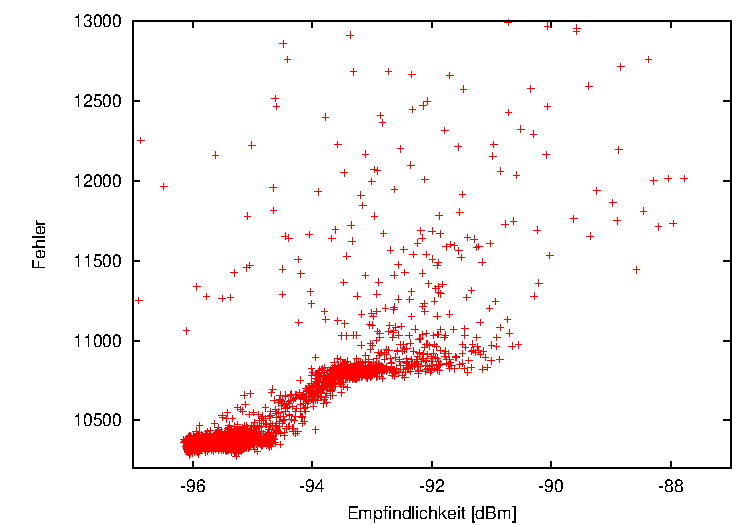
\includegraphics[width=0.6\linewidth]{Images/Chapter/bspgrafik1} % externe Grafik laden
% \caption{Dieses Diagramm ist ein Beispiel für eine einfache Abbildung.}\label{fig:testabb}
% \end{figure}


% Eine Abbildung sollte sich immer in einer Figure-Umgebung befinden.
% In dieser kann sie mit einer Caption beschrieben werden
% und sie kann über ein Label gekennzeichnet werden (vgl. Abbildung \ref{fig:testabb}).

% Dabei muss es keine Grafik sein, die in eine Figure-Umgebung geladen wird.
% Es kann dort ganz normal \LaTeX geschrieben werden,
% wie Abbildung \ref{fig:testabb2} zeigt.

% \begin{figure}
% \centering
% \fbox{\parbox{0.9\linewidth}{\centering In einer Figure muss keine Grafik stehen... Eine Abbildung kann im Prinzip alles sein.}}
% \caption{Dies ist eine Bildunterschrift} \label{fig:testabb2}
% \end{figure}

% \subsection{Unterabbildungen}

% \begin{figure}%
%   \centering
%    \subfloat[Die erste Unterabbildung]{\label{fig:subfig1}%
%        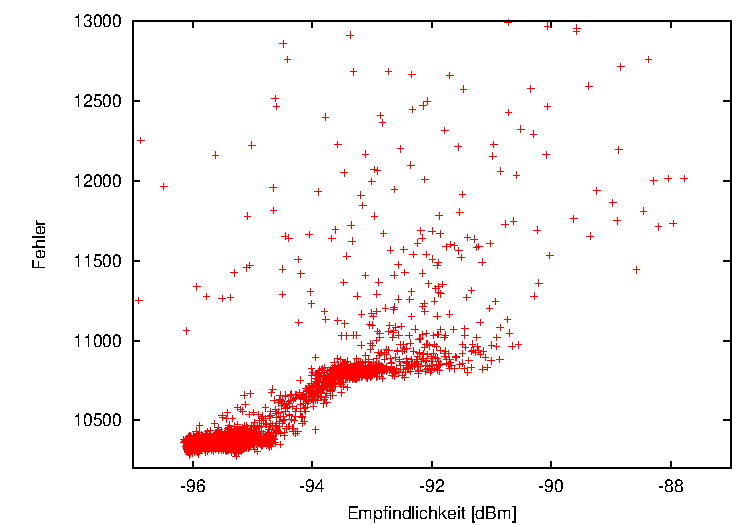
\includegraphics[width=0.48\linewidth]{Images/Chapter/bspgrafik1}
%    }\hfill
%    \subfloat[Die zweite Unterabbildung]{\label{fig:subfig2}%
%        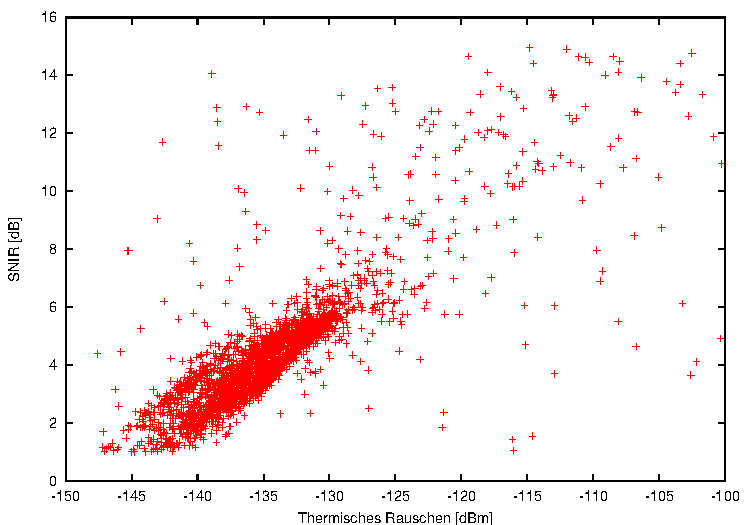
\includegraphics[width=0.48\linewidth]{Images/Chapter/bspgrafik2}
%    }
%    \caption{Beispiel für Unterabbildungen}
%    \label{fig:subfigexample}
% \end{figure}


% In manchen Fällen ist es sinnvoll eine Abbildung in Unterabbildungen zu teilen.
% In Abbildung \ref{fig:subfigexample} wird dies gezeigt.
% Die Abbildungen \ref{fig:subfig1} und \ref{fig:subfig2} sind Unterabbildungen.

% \section{Formeln}

% Für seinen Formelsatz ist \LaTeX besonders bekannt, weshalb es hier nicht an einem kleinen Beispiel (vgl. Formel \ref{eq::gewichtsumme}) fehlen soll.

% \begin{equation}
% f\idx{sim}(g,U)=\sum\limits^{n\idx{M}}_{\mu=1} w_\mu\cdot c_i( M_\mu(g,U)) \label{eq::gewichtsumme}
% \end{equation}

% \section{Quelltexte einbinden}

% \begin{figure}[t]
% \begin{lstlisting}[language=java, caption={Beispiel für ein Listing},  label=lst:bsplst]
% public class RadioFitness extends BasicFitness {
%   ...
%   SimResultReader result = new SimResultReader();
%   ...
%   protected void readResult(Scenario s) throws FitnessException {
%     result.readFrom(s.getExecEnv().getExecutionDir());
%   }

%   protected double getRawMetric(String name) throws FitnessException {
%     if(name.equals("delivery rate")
%       return result.getNumSendData()/result.getNumReceivedData();
%     else if(name.equals("latency"))
%       return results.getLatency();
%     else ...
%   } // comment
%   ...
% }
% \end{lstlisting}
% \end{figure}


% Ein Beispiel für ein Java-Listing zeigt Listing \ref{lst:bsplst}.


% \section{Zitieren von Quellen}

% Aussagen wollen gut belegt sein.
% Hier sind willkürlich \cite{FejF08} beispielhafte Zitierungen \cite{Deming1986} angegeben,
% die keinen inhaltlichen Bezug zu diesem Text aufweisen.
% Vielmehr geht es darum beispielhaft zu zitieren.
% Es können auch mehrere Quellen angegeben werden \cite{biturl,Rost2009} (auch hier wieder ohne inhaltlichen Bezug).

% Die Literaturangaben werden in einer Datenbank verwaltet,
% die in einer .bib-Datei gespeichert wird.
% In dieser kann auch nicht zitierte Literatur stehen.
% Eine gute Software zur Bearbeitung dieser Datenbank ist JabRef \cite{jabref}.